%File: formatting-instructions-latex-2024.tex
%release 2024.0
\documentclass[letterpaper]{article} % DO NOT CHANGE THIS
\usepackage{aaai24}  % DO NOT CHANGE THIS
\usepackage{times}  % DO NOT CHANGE THIS
\usepackage{helvet}  % DO NOT CHANGE THIS
\usepackage{courier}  % DO NOT CHANGE THIS
\usepackage[hyphens]{url}  % DO NOT CHANGE THIS
\usepackage{graphicx} % DO NOT CHANGE THIS
\urlstyle{rm} % DO NOT CHANGE THIS
\def\UrlFont{\rm}  % DO NOT CHANGE THIS
\usepackage{natbib}  % DO NOT CHANGE THIS AND DO NOT ADD ANY OPTIONS TO IT
\usepackage{caption} % DO NOT CHANGE THIS AND DO NOT ADD ANY OPTIONS TO IT
\frenchspacing  % DO NOT CHANGE THIS
\setlength{\pdfpagewidth}{8.5in}  % DO NOT CHANGE THIS
\setlength{\pdfpageheight}{11in}  % DO NOT CHANGE THIS
%
% These are recommended to typeset algorithms but not required. See the subsubsection on algorithms. Remove them if you don't have algorithms in your paper.
\usepackage{algorithm}
\usepackage{algorithmic}

%
% These are are recommended to typeset listings but not required. See the subsubsection on listing. Remove this block if you don't have listings in your paper.
\usepackage{newfloat}
\usepackage{listings}
\DeclareCaptionStyle{ruled}{labelfont=normalfont,labelsep=colon,strut=off} % DO NOT CHANGE THIS
\lstset{%
	basicstyle={\footnotesize\ttfamily},% footnotesize acceptable for monospace
	numbers=left,numberstyle=\footnotesize,xleftmargin=2em,% show line numbers, remove this entire line if you don't want the numbers.
	aboveskip=0pt,belowskip=0pt,%
	showstringspaces=false,tabsize=2,breaklines=true}
\floatstyle{ruled}
\newfloat{listing}{tb}{lst}{}
\floatname{listing}{Listing}
%
% Keep the \pdfinfo as shown here. There's no need
% for you to add the /Title and /Author tags.
\pdfinfo{
/TemplateVersion (2024.1)
}

% DISALLOWED PACKAGES
% \usepackage{authblk} -- This package is specifically forbidden
% \usepackage{balance} -- This package is specifically forbidden
% \usepackage{color (if used in text)
% \usepackage{CJK} -- This package is specifically forbidden
% \usepackage{float} -- This package is specifically forbidden
% \usepackage{flushend} -- This package is specifically forbidden
% \usepackage{fontenc} -- This package is specifically forbidden
% \usepackage{fullpage} -- This package is specifically forbidden
% \usepackage{geometry} -- This package is specifically forbidden
% \usepackage{grffile} -- This package is specifically forbidden
% \usepackage{hyperref} -- This package is specifically forbidden
% \usepackage{navigator} -- This package is specifically forbidden
% (or any other package that embeds links such as navigator or hyperref)
% \indentfirst} -- This package is specifically forbidden
% \layout} -- This package is specifically forbidden
% \multicol} -- This package is specifically forbidden
% \nameref} -- This package is specifically forbidden
% \usepackage{savetrees} -- This package is specifically forbidden
% \usepackage{setspace} -- This package is specifically forbidden
% \usepackage{stfloats} -- This package is specifically forbidden
% \usepackage{tabu} -- This package is specifically forbidden
% \usepackage{titlesec} -- This package is specifically forbidden
% \usepackage{tocbibind} -- This package is specifically forbidden
% \usepackage{ulem} -- This package is specifically forbidden
% \usepackage{wrapfig} -- This package is specifically forbidden
% DISALLOWED COMMANDS
% \nocopyright -- Your paper will not be published if you use this command
% \addtolength -- This command may not be used
% \balance -- This command may not be used
% \baselinestretch -- Your paper will not be published if you use this command
% \clearpage -- No page breaks of any kind may be used for the final version of your paper
% \columnsep -- This command may not be used
% \newpage -- No page breaks of any kind may be used for the final version of your paper
% \pagebreak -- No page breaks of any kind may be used for the final version of your paperr
% \pagestyle -- This command may not be used
% \tiny -- This is not an acceptable font size.
% \vspace{- -- No negative value may be used in proximity of a caption, figure, table, section, subsection, subsubsection, or reference
% \vskip{- -- No negative value may be used to alter spacing above or below a caption, figure, table, section, subsection, subsubsection, or reference

\setcounter{secnumdepth}{0} %May be changed to 1 or 2 if section numbers are desired.

% The file aaai24.sty is the style file for AAAI Press
% proceedings, working notes, and technical reports.
%

% Title

% Your title must be in mixed case, not sentence case.
% That means all verbs (including short verbs like be, is, using,and go),
% nouns, adverbs, adjectives should be capitalized, including both words in hyphenated terms, while
% articles, conjunctions, and prepositions are lower case unless they
% directly follow a colon or long dash
\title{Hierarchical Reinforcement Learning: Maze with Tasks}
\author{
    %Authors
    % All authors must be in the same font size and format.
    Rubén Cid Costa, Aimar Nicuesa Usandizaga, Daniel Obreo Sanz
}
\affiliations{
    %Afiliations
    Universidad Carlos III de Madrid 
    % If you have multiple authors and multiple affiliations
    % use superscripts in text and roman font to identify them.
    % For example,

    % Sunil Issar\textsuperscript{\rm 2}, 
    % J. Scott Penberthy\textsuperscript{\rm 3}, 
    % George Ferguson\textsuperscript{\rm 4},
    % Hans Guesgen\textsuperscript{\rm 5}
    % Note that the comma should be placed after the superscript

    Ronda de Toledo, 1. 28005 Madrid (Madrid). Spain
    % email address must be in roman text type, not monospace or sans serif
%
% See more examples next
}

%Example, Single Author, ->> remove \iffalse,\fi and place them surrounding AAAI title to use it
\iffalse
\title{My Publication Title --- Single Author}
\author {
    Author Name
}
\affiliations{
    Affiliation\\
    Affiliation Line 2\\
    name@example.com
}
\fi

\iffalse
%Example, Multiple Authors, ->> remove \iffalse,\fi and place them surrounding AAAI title to use it
\title{My Publication Title --- Multiple Authors}
\author {
    % Authors
    First Author Name\textsuperscript{\rm 1,\rm 2},
    Second Author Name\textsuperscript{\rm 2},
    Third Author Name\textsuperscript{\rm 1}
}
\affiliations {
    % Affiliations
    \textsuperscript{\rm 1}Affiliation 1\\
    \textsuperscript{\rm 2}Affiliation 2\\
    firstAuthor@affiliation1.com, secondAuthor@affilation2.com, thirdAuthor@affiliation1.com
}
\fi


% REMOVE THIS: bibentry
% This is only needed to show inline citations in the guidelines document. You should not need it and can safely delete it.
\usepackage{bibentry}
% END REMOVE bibentry

\begin{document}

\maketitle

\begin{abstract}
En este documento se detalla el estudio teórico y la evaluación práctica del dominio de Aprendizaje por Refuerzo Jerárquico. El problema estudiado es el Maze With Tasks, que consiste en resolver un laberinto en el que se deben realizar acciones intermedias. Se empleará como técnica el Aprendiaje por Refuerzo Feudal, que se basa en un sistema jerárquico en el que un sistema toma decisiones a alto nivel y otra serie de subsistemas realizan acciones a más bajo nivel.
\end{abstract}


\section{Introducción}
En el campo de la IA, y su rápida evolución, el aprendizaje por refuerzo ha surgido como una herramienta poderosa para los problemas que implican toma de decisiones. Desde que se crearon, quedo demostrado su éxito notable en tareas de dicho tipo desde juegos hasta robótica. Sin embargo, a medida que las tareas se vuelven más complejas el uso de un solo algoritmo se ve influenciado debido a las limitaciones de los enfoques de AR planos. Es entonces cuando se ve la necesidad de ofrecer sistemas que dividan el problema en subtareas más manejables, los modelos de Aprendizaje de Refuerzo Jerárquico (ARJ).

El aprendizaje por refuerzo jerárquico introdujo la estructura jerárquica al proceso de aprendizaje. Debido a ello, en vez de aprender una política para asignar el estado directamente a acciones, el ARJ permite aprender diferentes niveles de políticas, otorgando diferentes niveles de abstracción al sistema. Debido a ello, permite dividir la tarea inicial en tantas tareas como sean necesarias para enfrentar la complejidad del problema a resolver. Estas características no solo otorgan mayor nivel de simplicidad a cada política si no que ofrecen también una mejor escalabilidad y eficiencia a los algoritmos creados.

Uno de los problemas típicos de dichas arquitecturas es el “Maze with Tasks” que consisten en problemas de laberintos de tareas. En dicha tarea tenemos como objetivo enseñar a un agente a navegar y completar múltiples objetivos dentro de un laberinto. Debida a la multitud de tareas que tiene que realizar el agente para poder lograr la navegación correcta por el laberinto, el problema se divide en diferentes subtareas jerárquicas (unas dependen de otras) que mediante la combinación permiten obtener el resultado esperado.

Dentro de la jerarquía, las tareas a realizar se dividen en diferentes niveles de abstracción, donde la ejecución de una tarea influencia de forma directa la ejecución de las tareas hijas. Un agente de alto nivel (el meta-controlador) decide que subtareas u opción debe ejecutarse a continuación (tareas a realizar a largo plazo). Dicha elección pasa al nivel inferior donde los controladores deciden las acciones especificas necesarias para completar esa subtarea (tareas cuya ejecución es momentánea). En dichas tareas es tan importante la definición de la jerarquía como el equilibrio entre la explotación de nuevas estrategias y la explotación del conocimiento adquirido para que la recompensa a largo plazo sea máxima.

De entre las arquitecturas de los ARJ, debido a la estructura jerárquica que comparte con los sistemas que regían en la Edad Media, son particularmente útiles los algoritmos de Aprendizaje por Refuerzo Feudal (ARF) para solventar dichos problemas. En el problema un gerente de alto nivel asigna la tarea a realizar a continuación mientras que los otros subgerentes reciben la tarea de realizar las acciones necesarias para lograr el fin propuesto.
\cite {geeksforgeeks2024hrl,sutton1999between,barto2003recent,dietterich2000hierarchical}
\section{Estudio teórico}

\subsection{FeUdal Networks: FuN}

Las redes feudales se basan en la arquitectura de aprendiaje por refuerzo feudal, 
una arquitectura del aprendizaje por refuerzo jerárquico. Esta arquitectura emplea un sistema de control, conocido
como "manager", que asigna tareas a un subsistema conocido como "worker" que debe aprender a ejecutarlas de manera óptima.

La arquitectura del sistema se muestra en la imagen siguiente \cite{feudal_networks_2024}.

\begin{figure}[H]
    \centering
    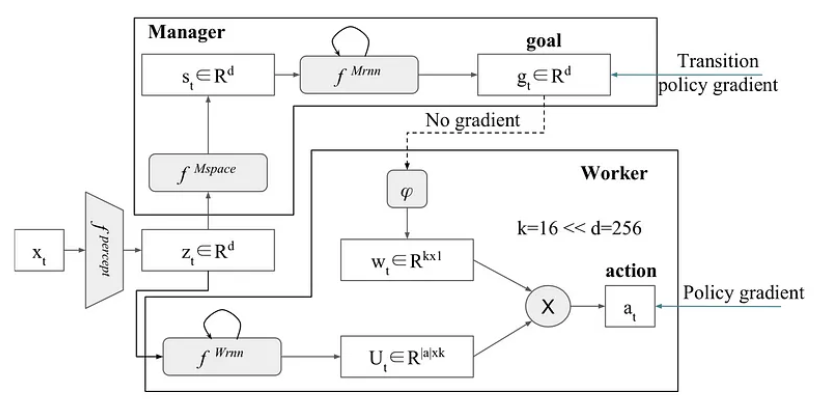
\includegraphics[width=0.9\columnwidth]{feudal_arquitecture.png}
    \caption{Arquitectura de una red feudal.}
    \label{fig:arquitectura_feudal}
\end{figure}

La entrada de esta red es procesada por una capa de percepción, que emplea capas convolucionales
para extraer características de la imagen de entrada. A continuación, estas características son procesadas
tanto por el worker como por el manager, cada uno de manera distinta; el manager extrae objetivos y el worker
aprende a alcanzar esos objetivos.

El objetivo principal del manager es generar metas que el worker debe cumplir. Recibe la percepción
del entorno, proporcionada por el módulo de percepción, ese estado es procesado por una red recurrente LSTM
para mantener un estado interno y poder capturar información relevante en horizontes temporales largos.
El manager emplea esta información para predecir un objetivo direccional en el espacio latente, este objetivo
es un vector unitario, lo que asegura que el worker se enfoque en la dirección y no en la posición absoluta.

Para entrenar el manager, se emplea la recompensa obtenida, y emplea la similitud coseno entre la dirección en la que 
se movió el worker y la compara con el objetivo establecido, empleando la similitud coseno como función de pérdida.
Esta pérdida incentiva al Manager a emitir objetivos que maximicen el progreso hacia estados ventajosos.

El vector de objetivos se envía al worker sin propagar gradientes, esto garantiza que los objetivos 
mantengan un significado semántico independiente, en lugar de ser simples variables latentes optimizadas de manera conjunta.

En el caso del worker, también se emplea una red LSTM para mantener un estado interno y poder capturar información relevante,
pero en este caso, el worker recibe tanto la percepción del entorno como el objetivo del manager. El worker emplea esta información
para predecir la acción que debe realizar para alcanzar el objetivo. La acción se predice en el espacio de acciones, y se emplea


\subsection{Definición}

\subsection{Estado del arte}

\section{Evaluación práctica}

\section{Conclusiones}





\bibliography{aaai24}

\end{document}
